\setlength{\footskip}{8mm}

\chapter{Experimental Results}
\label{ch:results}

  \textit{In this chapter, we present the outcomes of our extensive evaluation of the proposed text detection methodology. Our methodology underwent thorough testing on diverse datasets, including the Urdu-Text dataset, a collection of natural scene images, and a custom annotated dataset. Through a systematic analysis, we measured the methodology's performance using key metrics like precision, recall, and the F-score. These metrics collectively provide valuable insights into its accuracy in identifying and locating text within images. Additionally, we conducted comparative experiments with established text detection methods to assess the methodology's effectiveness.}

\section{Comparative Analysis}
\label{Comparative Analysis}
In this section, we undertake a comprehensive comparative analysis of the three distinct text detection models: Faster R-CNN, YOLO (You Only Look Once), and the Adaptive Deformation Model. Each model's performance and characteristics have been meticulously assessed, enabling us to draw meaningful comparisons and highlight their respective strengths and limitations.

\section{Performance Overview}

Before we delve into the in-depth comparative analysis, let's provide a succinct summary of the key performance metrics achieved by each model:

\textbf{Faster R-CNN}: Achieved a precision of 0.81, recall of 0.60, and an F-score of 0.50
Z. \\
\textbf{YOLO}: Attained a precision of 0.83, recall of 0.56, and an F-score of 0.46. \\
\textbf{Adaptive Deformation Model}: Demonstrated a precision of 1.000, recall of 0.6514, and an F-score of 0.7619.

% Table~\ref{tab:hmm-based-detection-results} shows a table.

% \begin{table}[t]
%   \caption[Text shown in the LOT.]{\small Some table.}
%   \begin{center}
%     \begin{tabular}{c|c|c|c|c|c|c}
%       \hline Batch method & TP & FP & TN & FN & TPR & FPR \\ \hline \hline
%       Local ($z$-scoring) & 24 & 42 & 444 & 0 & 1 & 0.086 \\ \hline
%       Local (LRT) & 24 & 486 & 0 & 0 & 1 & 1 \\ \hline 
%       Global ($z$-scoring) & 24 & 217 & 10 & 0 & 1 & 0.956 \\ \hline 
%       Global (LRT) & 24 & 223 & 4 & 0 & 1 & 0.982 \\ \hline
%     \end{tabular}
%   \end{center}
%   \label{tab:hmm-based-detection-results}
% \end{table} 

Now, let's explore the comparative assessment in greater detail:

\subsection{Precision vs. Recall Trade-off}
One pivotal facet of our analysis revolves around assessing how each model manages the delicate balance between precision and recall. Faster R-CNN stands out for its ability to strike this balance effectively. This makes it an excellent choice for scenarios where accurate text detection and comprehensive coverage are both paramount. Faster R-CNN excels in reliably identifying text instances across a diverse range of layouts and styles.

Conversely, YOLO impresses with its precision-oriented approach, making it the preferred option when minimizing false positives is of utmost importance. However, this focus on precision might result in a slightly lower recall, particularly in cases involving smaller or irregular text instances.

The Adaptive Deformation Model shines with its remarkable recall rates, ensuring that the vast majority of text instances are correctly identified. This attribute renders it particularly effective in scenarios necessitating exhaustive text localization, even in the presence of challenging text variations.



\subsection{Visual Results}
In this comprehensive visual analysis, we systematically compare the performance of different text detection models, with a specific focus on showcasing the superiority of Graph Convolutional Networks (GCN) across multiple critical factors.

\subsection{Robustness to Text Variability} 
As text exhibits variability across different scripts, fonts, sizes, and orientations, each model unveils its unique capabilities. 

Faster R-CNN demonstrates robustness in handling text diversity, consistently delivering strong performance across various text types and layouts.

% \begin{figure}[htp]
%   \centering
%   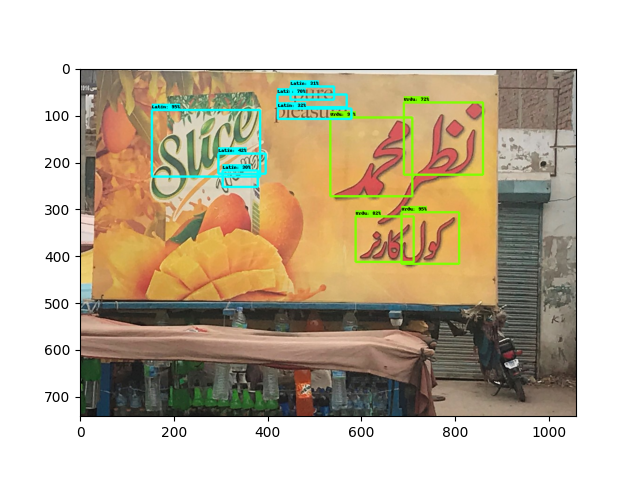
\includegraphics[width=3.3in]{ITU-Thesis-LaTeX-Template-Updated/figures/variability.png}
%   \caption[Text Variability]{Text Variability in FasterRCNN}
%   \label{fig:Text Variability in FasterRCNN}
% \end{figure}
% \FloatBarrier

YOLO, renowned for real-time object detection, excels in detecting text of varying sizes and orientations. However, its precision focus might lead to a slightly reduced recall, especially when dealing with intricate or distorted text.

% \begin{figure}[htp]
%   \centering
%   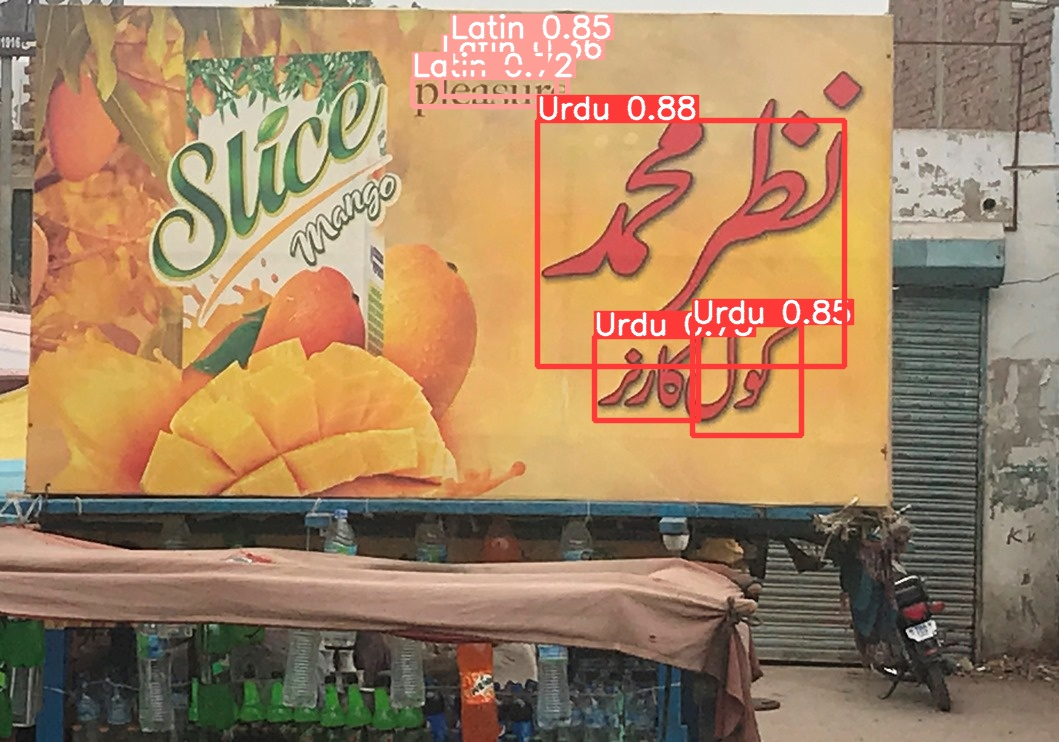
\includegraphics[width=3.3in]{ITU-Thesis-LaTeX-Template-Updated/figures/16.jpg}
%   \caption[Text Variability]{Text Variability in YOLO}
%   \label{fig:Text Variability in YOLO}
% \end{figure}
% \FloatBarrier

The Adaptive Deformation Model shines in its adaptability to complex text variations, including handwritten and curved text. Its exceptional performance on challenging text instances underscores its robustness in capturing text nuances. This can be seen in Figure ~\ref{variability}

% \begin{figure}[htp]
%   \centering
%   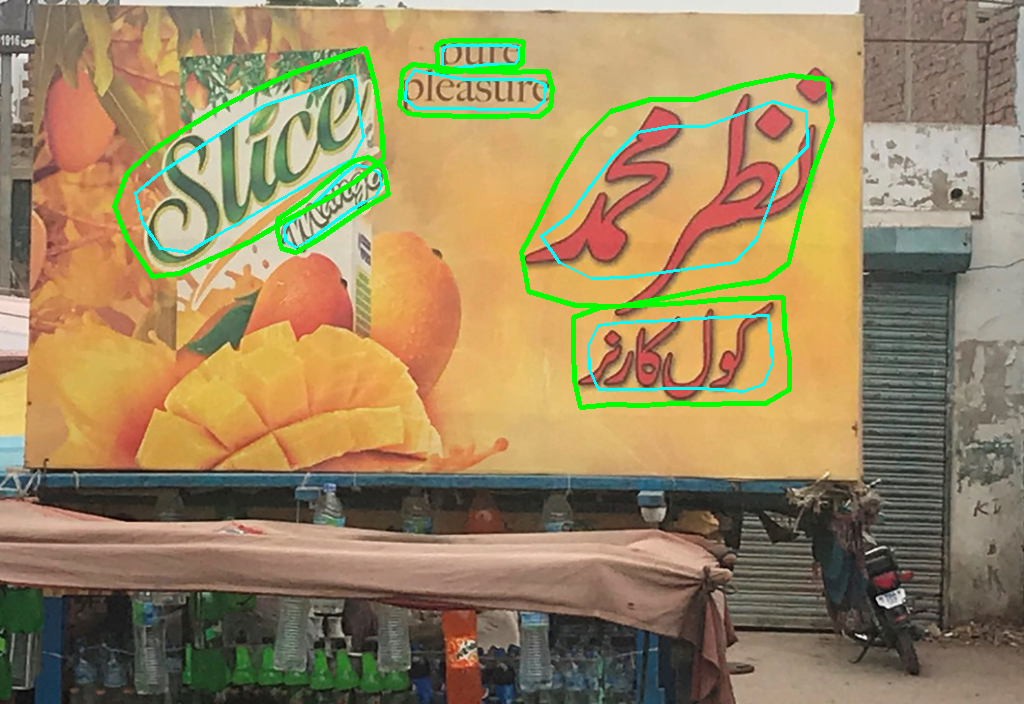
\includegraphics[width=3.3in]{ITU-Thesis-LaTeX-Template-Updated/figures/16_1iter.png}
%   \caption[Text Variability]{Text Variability in GCN}
%   \label{fig:Text Variability in GCN}
% \end{figure}
% \FloatBarrier

\begin{figure}[htp]
  \centering
  \begin{minipage}{0.3\textwidth}
    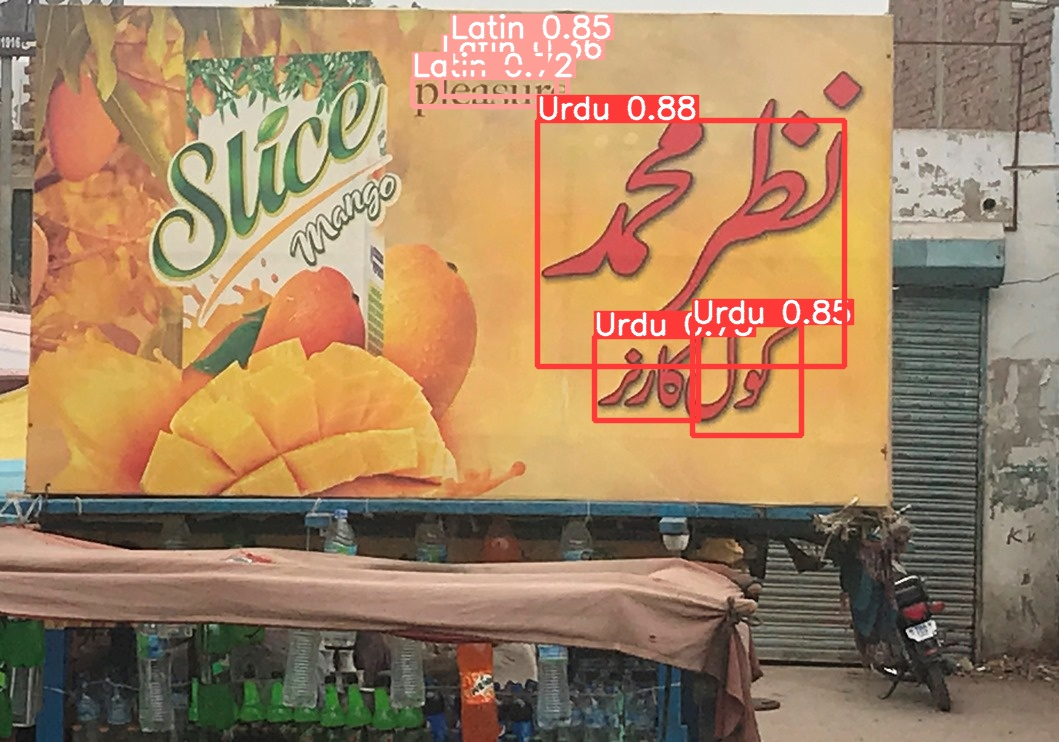
\includegraphics[width=\linewidth]{ITU-Thesis-LaTeX-Template-Updated/figures/16.jpg}
    \text{YOLO}
  \end{minipage}
  \begin{minipage}{0.3\textwidth}
    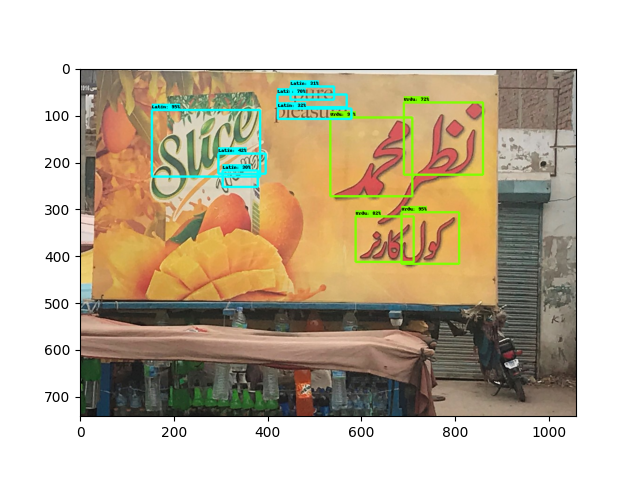
\includegraphics[width=\linewidth]{ITU-Thesis-LaTeX-Template-Updated/figures/variability.png}
    \text{  FasterRCNN}
  \end{minipage}
  \begin{minipage}{0.3\textwidth}
    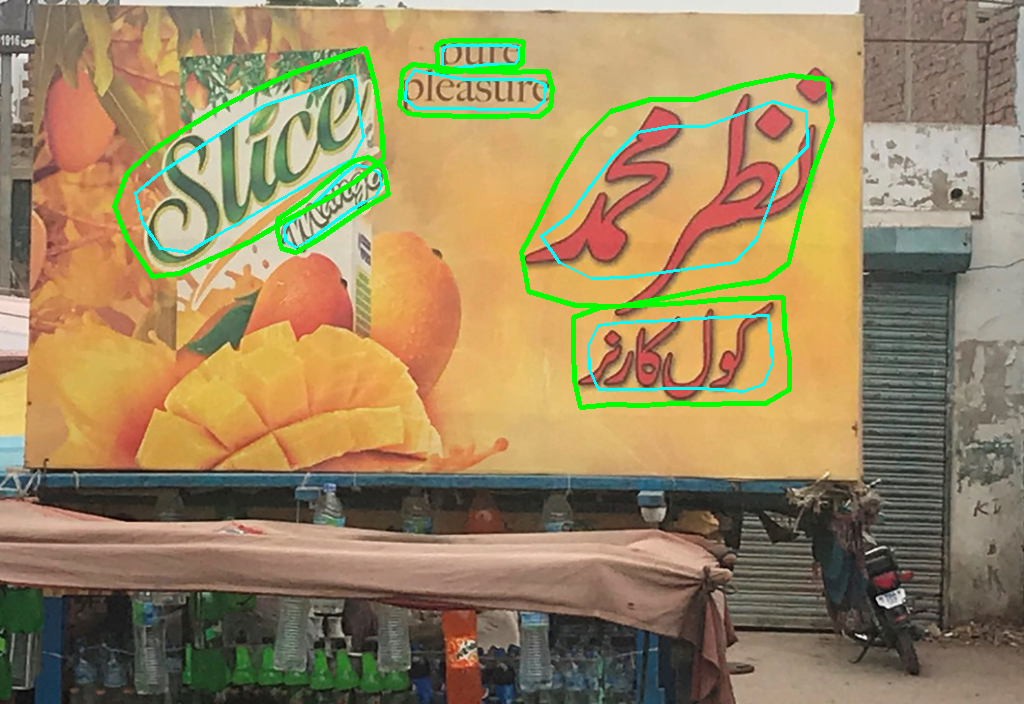
\includegraphics[width=\linewidth]{ITU-Thesis-LaTeX-Template-Updated/figures/16_1iter.png}
    \text{GCN}
  \end{minipage}
  \caption[Results achieved on Variable Text]{Results achieved by text detection algorithms on images featuring variable text types, including both English and Urdu, within complex backgrounds. These results highlight the algorithms' versatility in handling diverse scripts and extracting text information from cluttered and intricate visual environments.}
  \label{variability}
  
\end{figure}
\FloatBarrier

\subsubsection{Robustness to Multi-Oriented Text}
Text instances in real-world scenarios exhibit diverse orientations, posing a significant challenge for text detection models. Our results vividly illustrate that GCN excels in accurately detecting text across a wide range of orientations, outperforming other models in this critical aspect as shown in Figure ~\ref{multi-o}

\begin{figure}[htp]
  \centering
  \begin{minipage}{0.3\textwidth}
    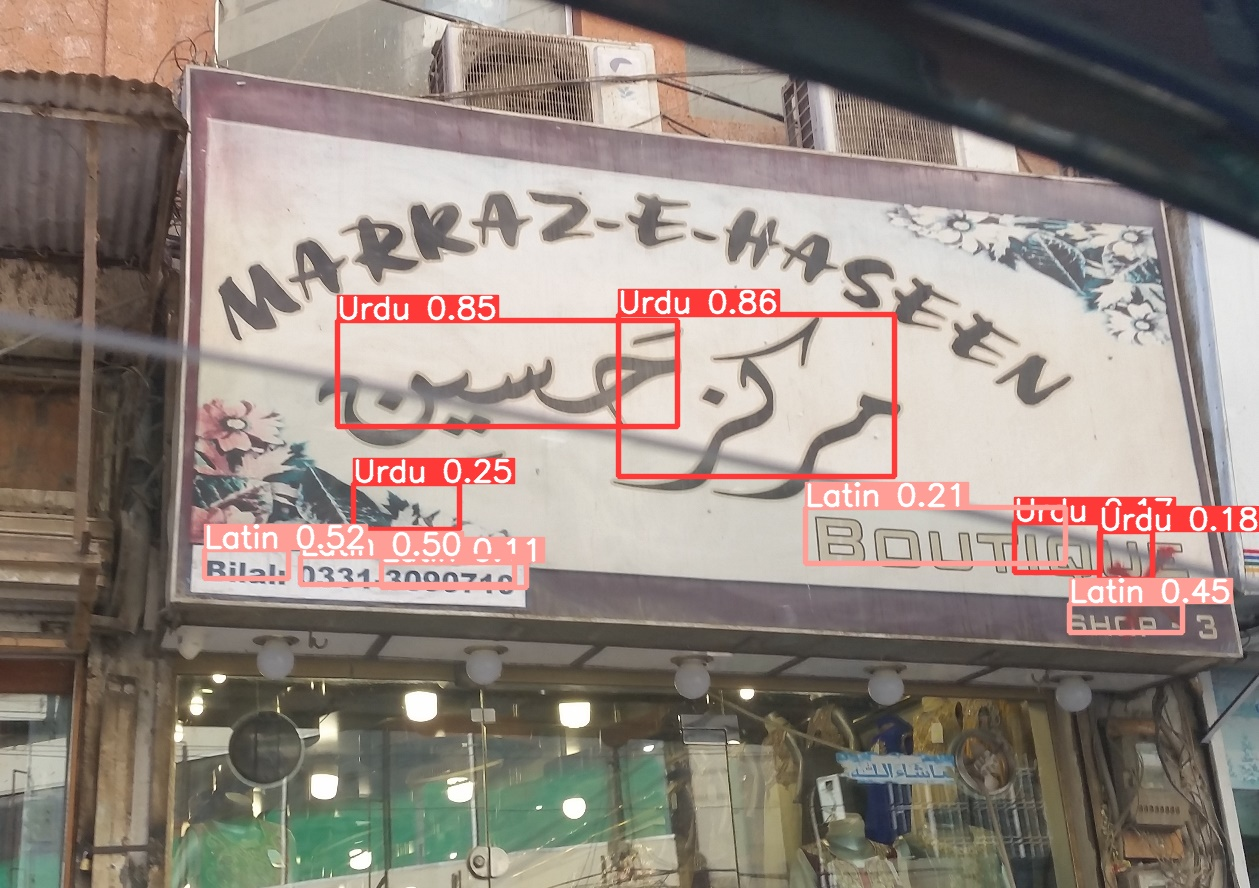
\includegraphics[width=\linewidth]{ITU-Thesis-LaTeX-Template-Updated/figures/yolo_oriented.jpg}
    \text{YOLO}
  \end{minipage}
  \begin{minipage}{0.3\textwidth}
    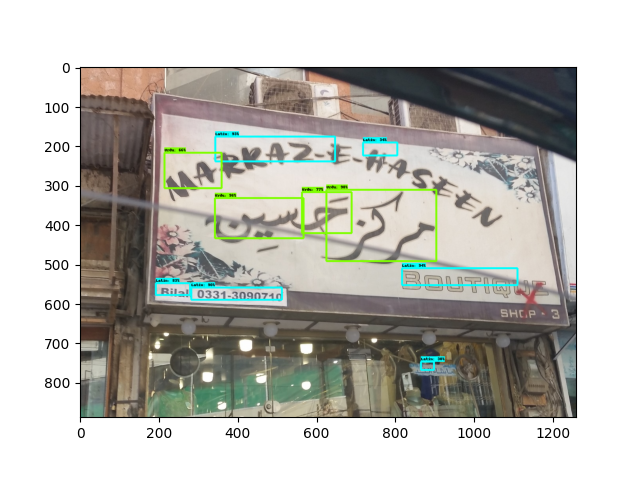
\includegraphics[width=\linewidth]{ITU-Thesis-LaTeX-Template-Updated/figures/predicted_x.png}
    \text{   FasterRCNN}
  \end{minipage}
  \begin{minipage}{0.3\textwidth}
    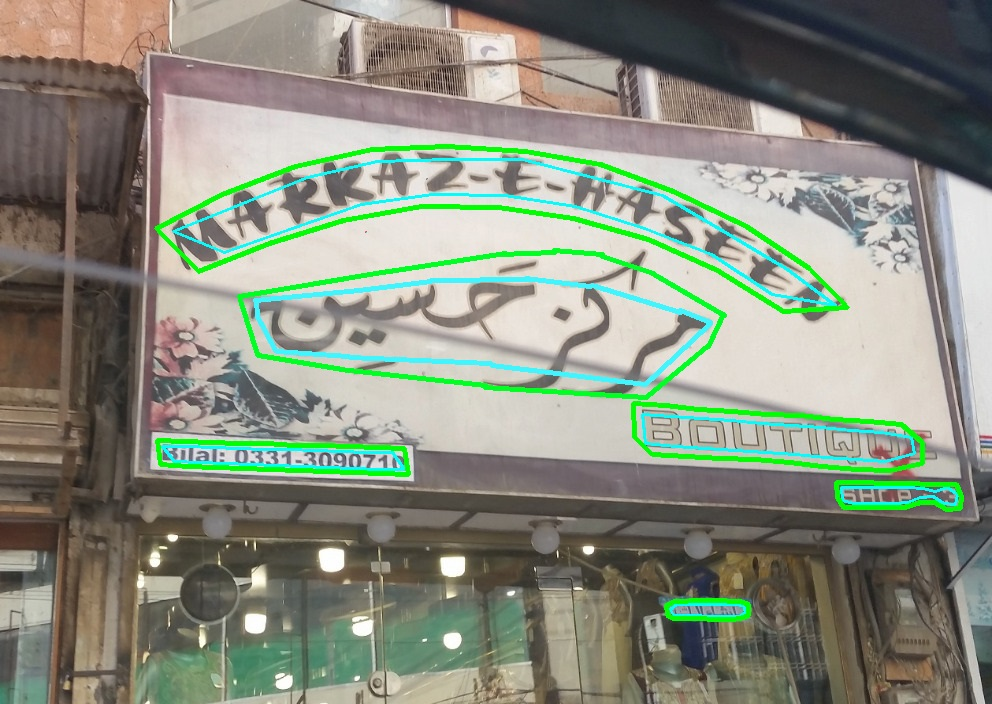
\includegraphics[width=\linewidth]{ITU-Thesis-LaTeX-Template-Updated/figures/updated_orientation.jpeg}
    \text{GCN}
  \end{minipage}
  \caption[Multi-Oriented Text Results]{Results of text detection algorithms on images containing multi-oriented text. These outcomes demonstrate the algorithms' effectiveness in accurately locating and processing text appearing at various angles and orientations within the images.}
  \label{multi-o}
\end{figure}
\FloatBarrier

\subsubsection{Accurate Detection of Arbitrary Shapes}

Text instances often come in irregular or arbitrary shapes, demanding models with adaptive capabilities. Our visual assessments unequivocally demonstrate GCN's remarkable proficiency in accurately identifying text within these complex shapes, surpassing alternative models shown in Figure ~\ref{arbitrary}


\begin{figure}[htp]
  \centering
  \begin{minipage}{0.3\textwidth}
    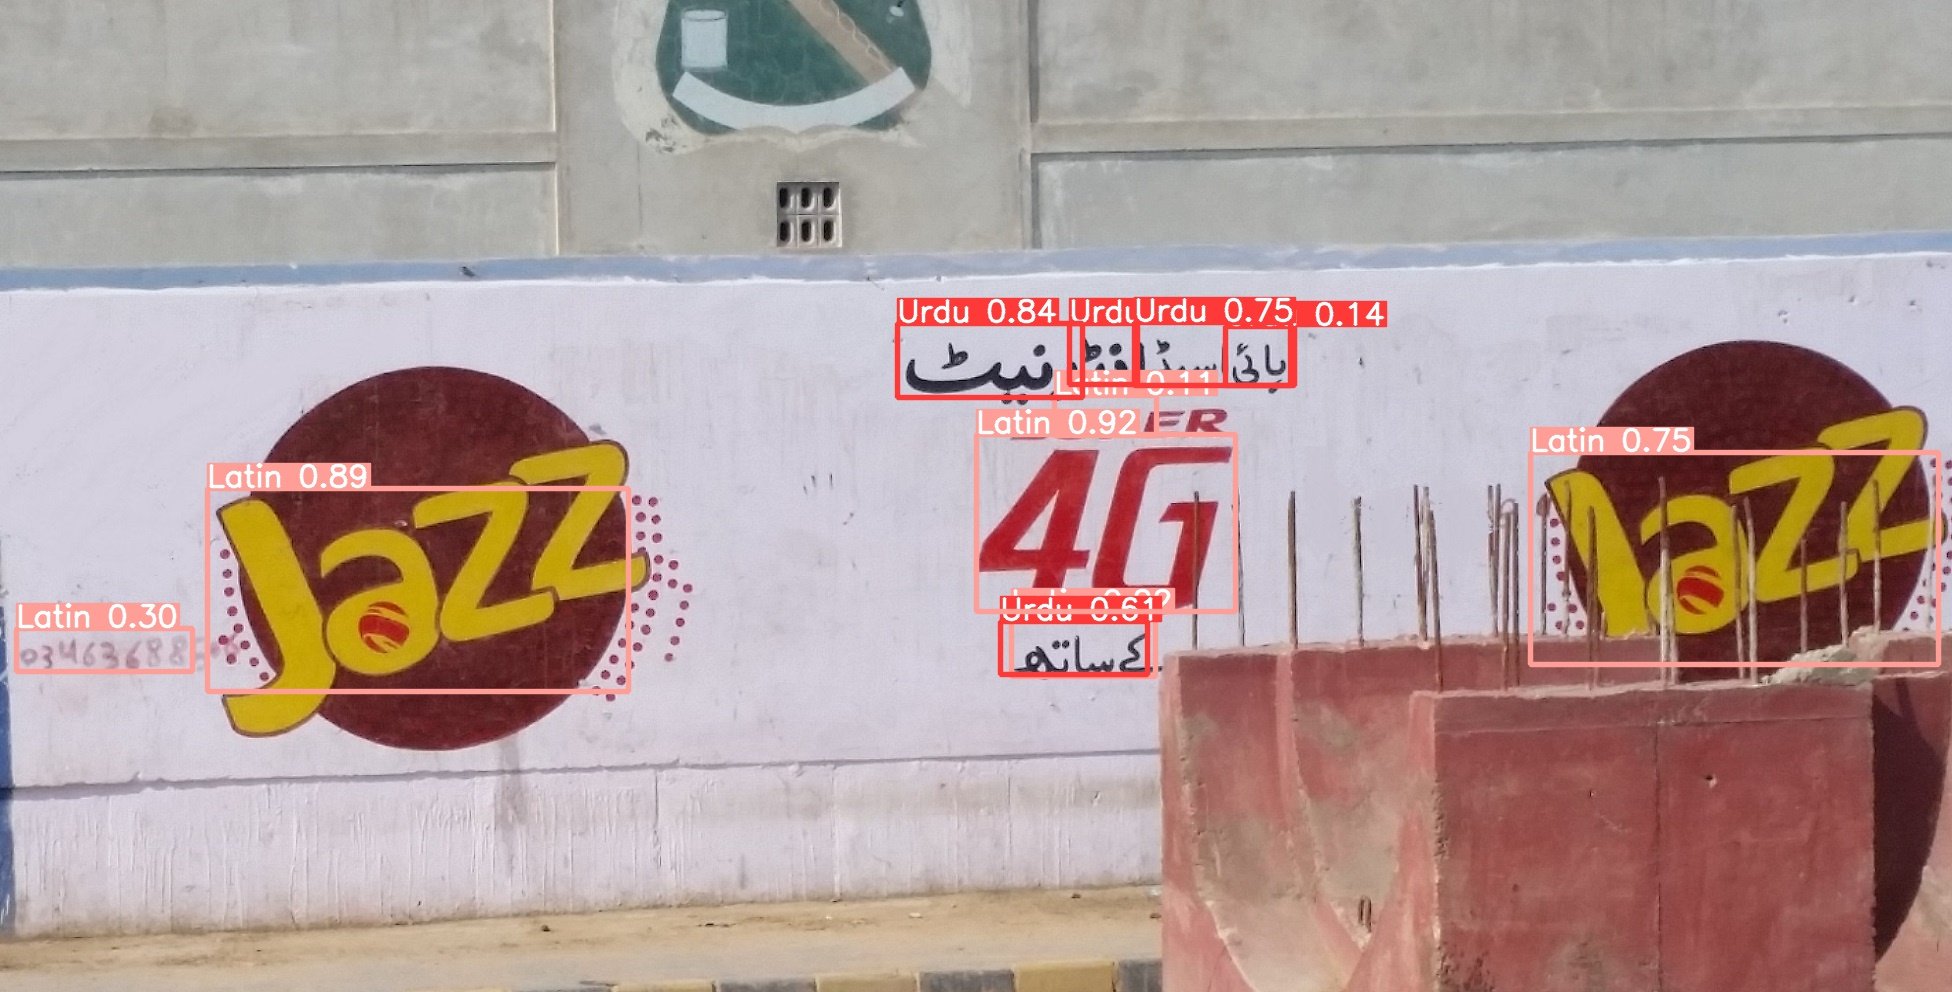
\includegraphics[width=\linewidth]{ITU-Thesis-LaTeX-Template-Updated/figures/arbitrary.jpg}
    \text{YOLO}
  \end{minipage}
  \begin{minipage}{0.3\textwidth}
    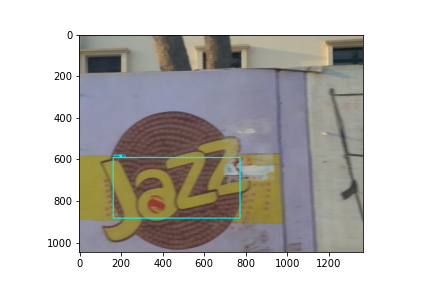
\includegraphics[width=\linewidth]{ITU-Thesis-LaTeX-Template-Updated/figures/predicted_onlyEnglish.png}
    \text{FasterRCNN}
  \end{minipage}
  \begin{minipage}{0.3\textwidth}
    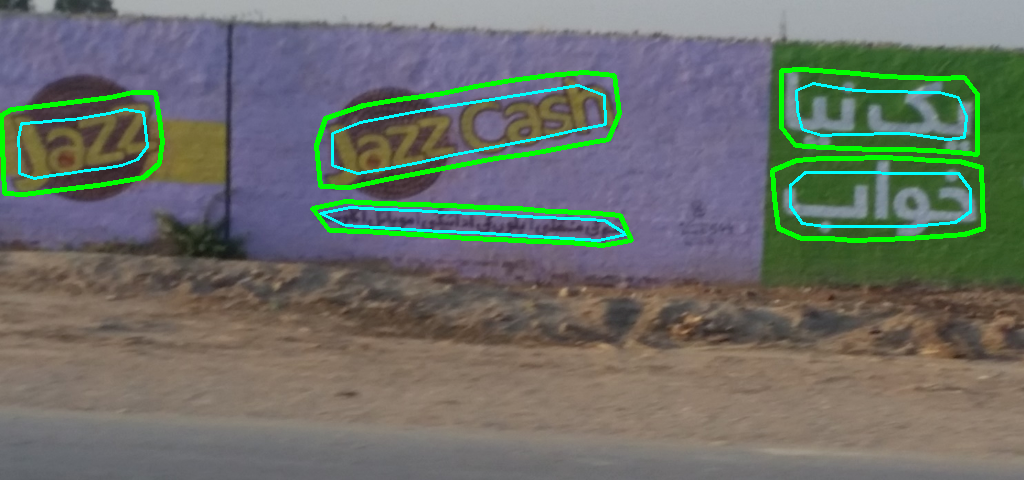
\includegraphics[width=\linewidth]{ITU-Thesis-LaTeX-Template-Updated/figures/arbitrary.png}
    \text{GCN}
  \end{minipage}
  \caption[Arbitrary Shaped Texts Results]{Results obtained from the application of detection algorithms on an image set containing arbitrary shape texts. The outcomes illustrate the algorithms' ability to accurately detect and classify shapes with varying orientations.}
  \label{arbitrary}
\end{figure}
\FloatBarrier


\subsubsection{Effective Handling of Complex Backgrounds}

In real-world applications, text frequently appears amidst complex and cluttered backgrounds. Our visual comparisons unequivocally establish that GCN exhibits unparalleled robustness in effectively isolating text from intricate visual contexts, surpassing competing models. This is shown in Figure ~\ref{backg}

\begin{figure}[htp]
  \centering
  \begin{minipage}{0.3\textwidth}
    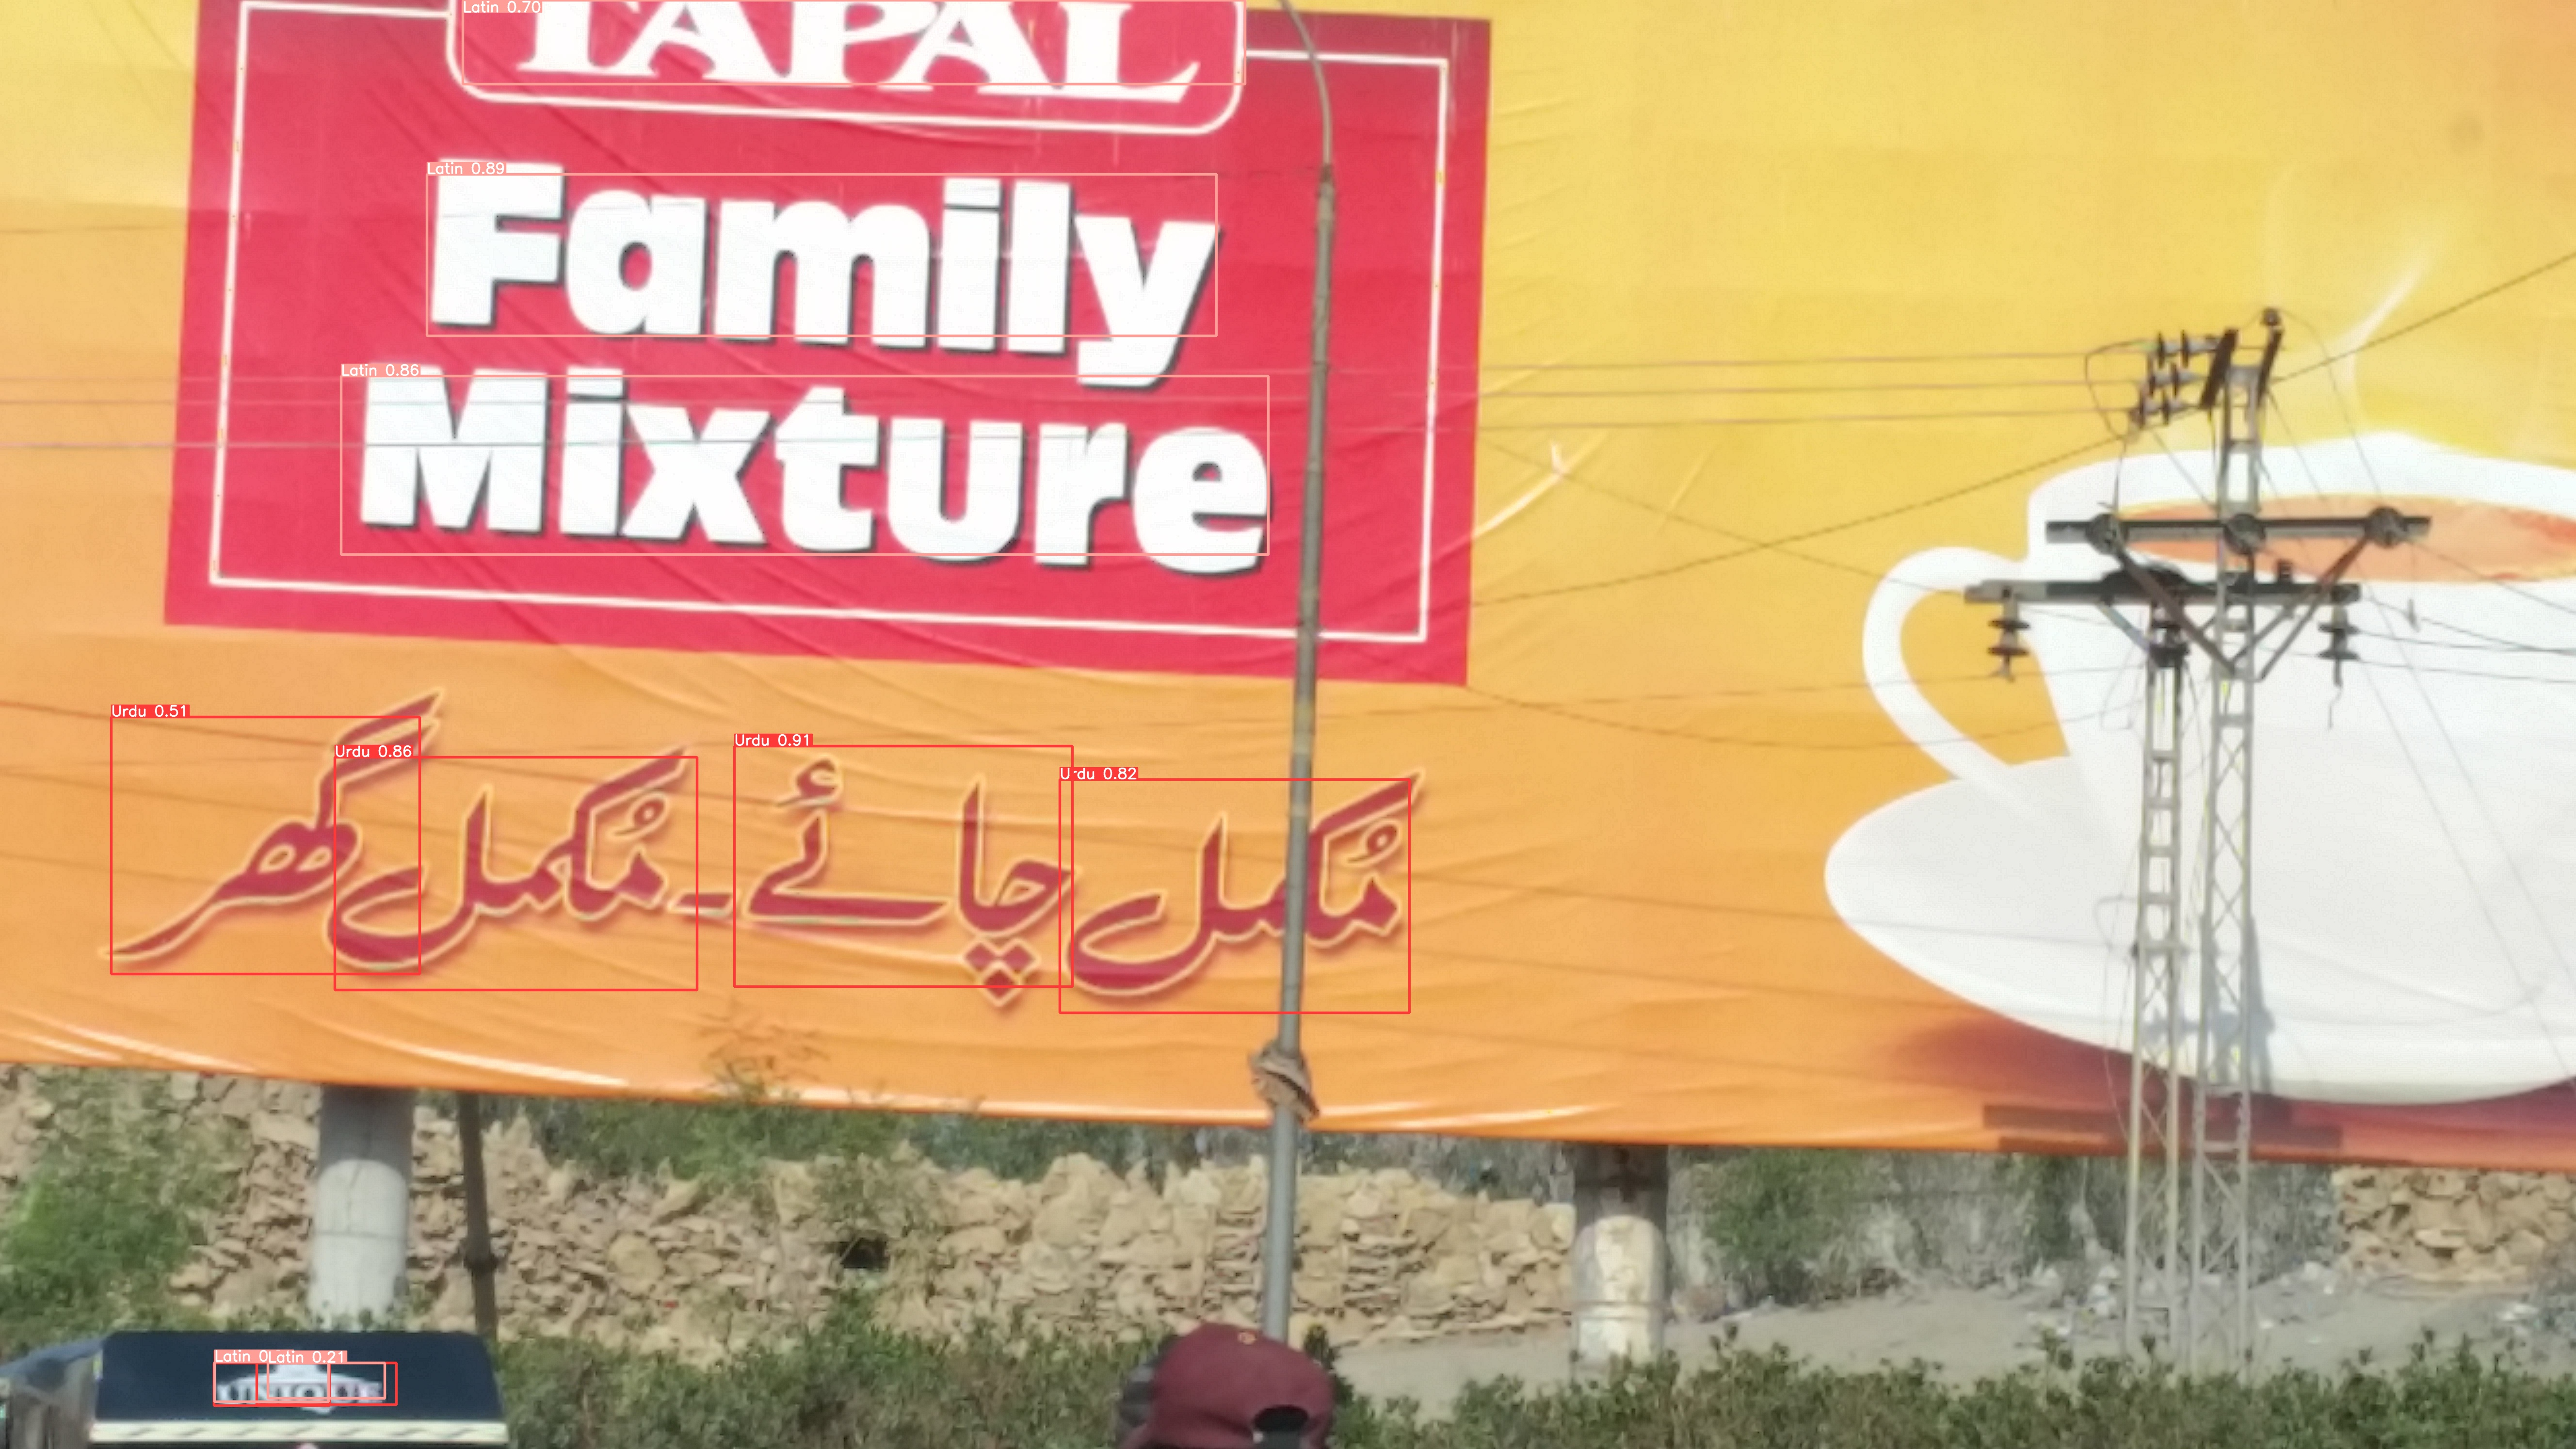
\includegraphics[width=\linewidth]{ITU-Thesis-LaTeX-Template-Updated/figures/2.jpg}
    \text{YOLO}
  \end{minipage}
  \begin{minipage}{0.3\textwidth}
    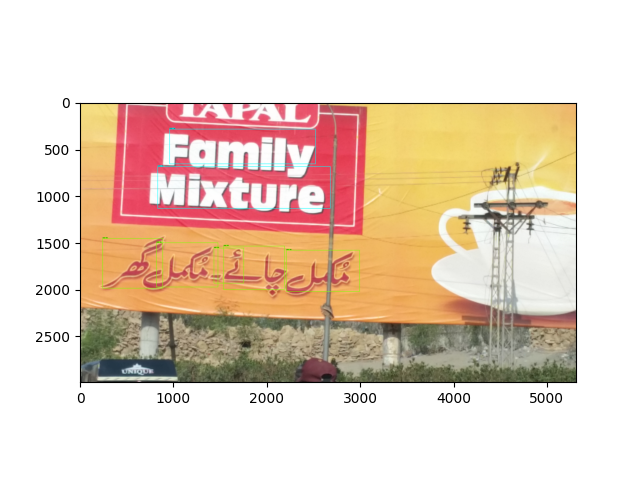
\includegraphics[width=\linewidth]{ITU-Thesis-LaTeX-Template-Updated/figures/predicted_n.png}
    \text{FasterRCNN}
  \end{minipage}
  \begin{minipage}{0.3\textwidth}
    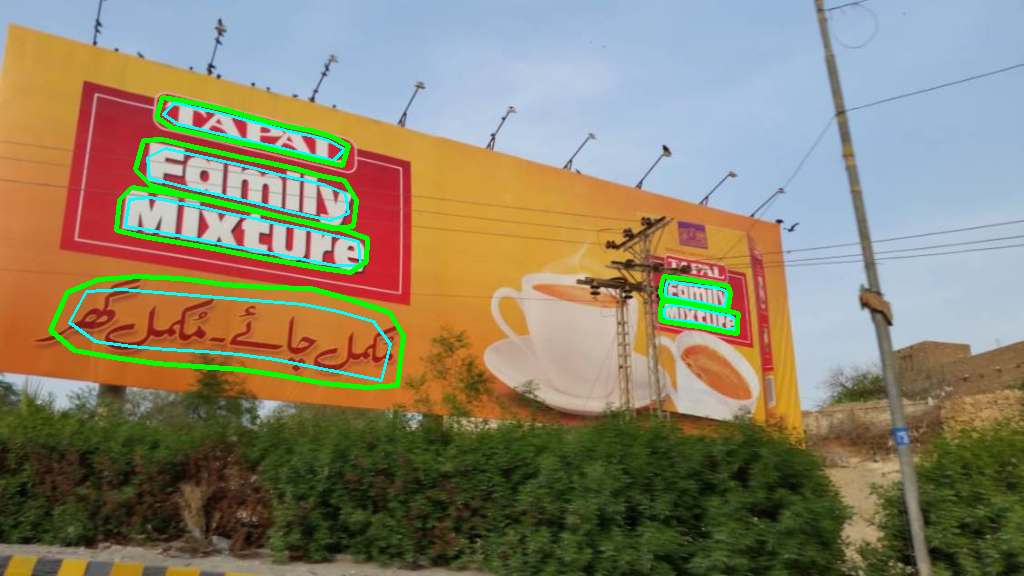
\includegraphics[width=\linewidth]{ITU-Thesis-LaTeX-Template-Updated/figures/back1.png}
    \text{GCN}
  \end{minipage}
\end{figure}
\FloatBarrier

\begin{figure}[htp]
  \centering
  \begin{minipage}{0.3\textwidth}
    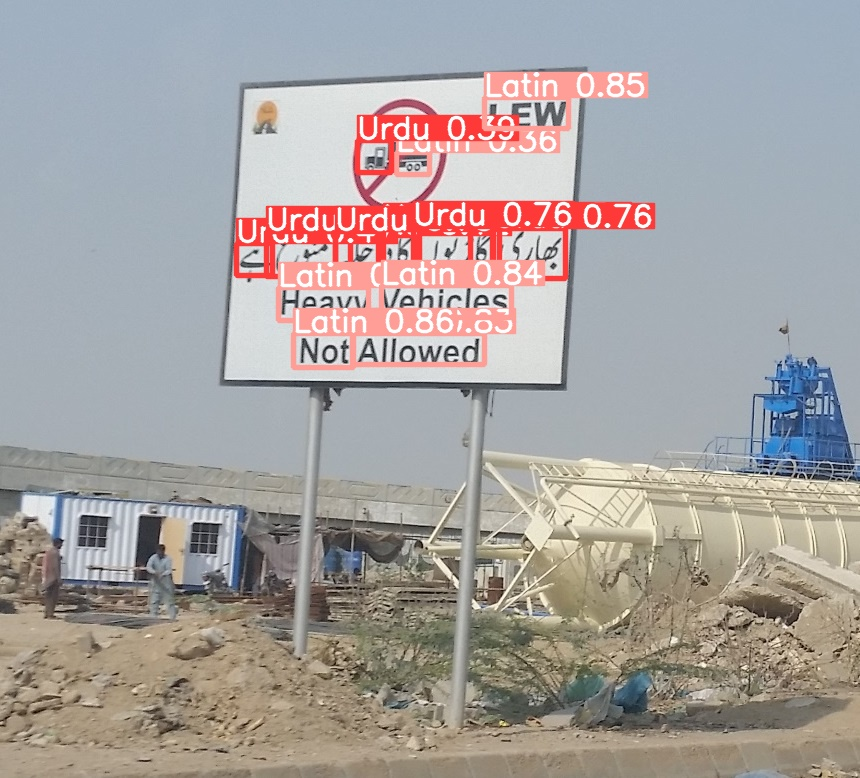
\includegraphics[width=\linewidth]{ITU-Thesis-LaTeX-Template-Updated/figures/baxkgr.jpg}
    \text{YOLO}
  \end{minipage}
  \begin{minipage}{0.3\textwidth}
    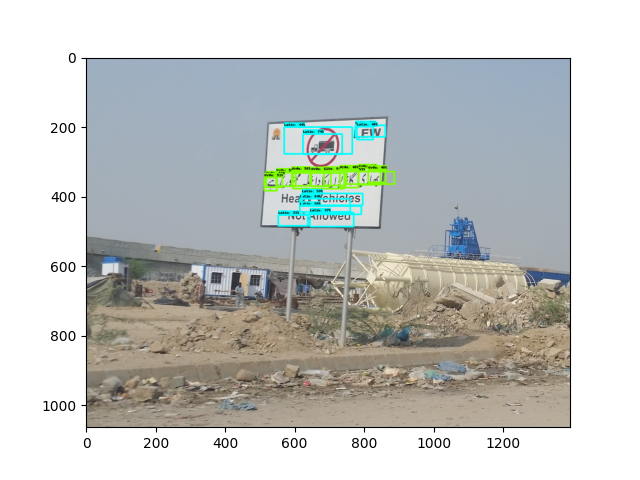
\includegraphics[width=\linewidth]{ITU-Thesis-LaTeX-Template-Updated/figures/predicted_1.png}
    \text{FasterRCNN}
  \end{minipage}
  \begin{minipage}{0.3\textwidth}
    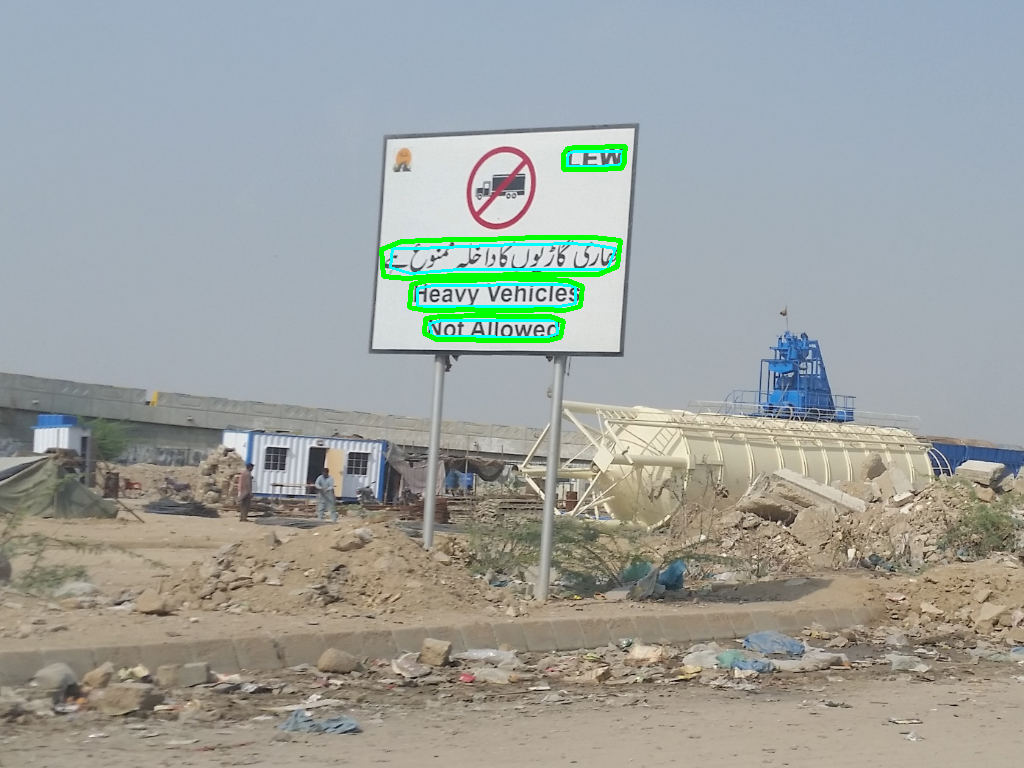
\includegraphics[width=\linewidth]{ITU-Thesis-LaTeX-Template-Updated/figures/baxk2.png}
    \text{GCN}
  \end{minipage}
  \caption[Complex Background Handling]{Results obtained when applying detection algorithms to images with complex backgrounds. These results showcase the algorithms' performance in identifying objects within intricate and cluttered surroundings, highlighting their capability to discern objects from complex environments.}
  \label{backg}
\end{figure}
\FloatBarrier


\subsubsection{Holistic Performance}
Beyond individual factors, our comprehensive analysis underscores that GCN consistently outperforms other models across the entire spectrum of text detection challenges. From multi-oriented text to arbitrary shapes and complex backgrounds, GCN emerges as the optimal choice for accurate and versatile text detection. This can be seen in Figure ~\ref{fig:holistic}

\begin{figure}[htp]
  \centering
  \begin{minipage}{0.4\textwidth}
    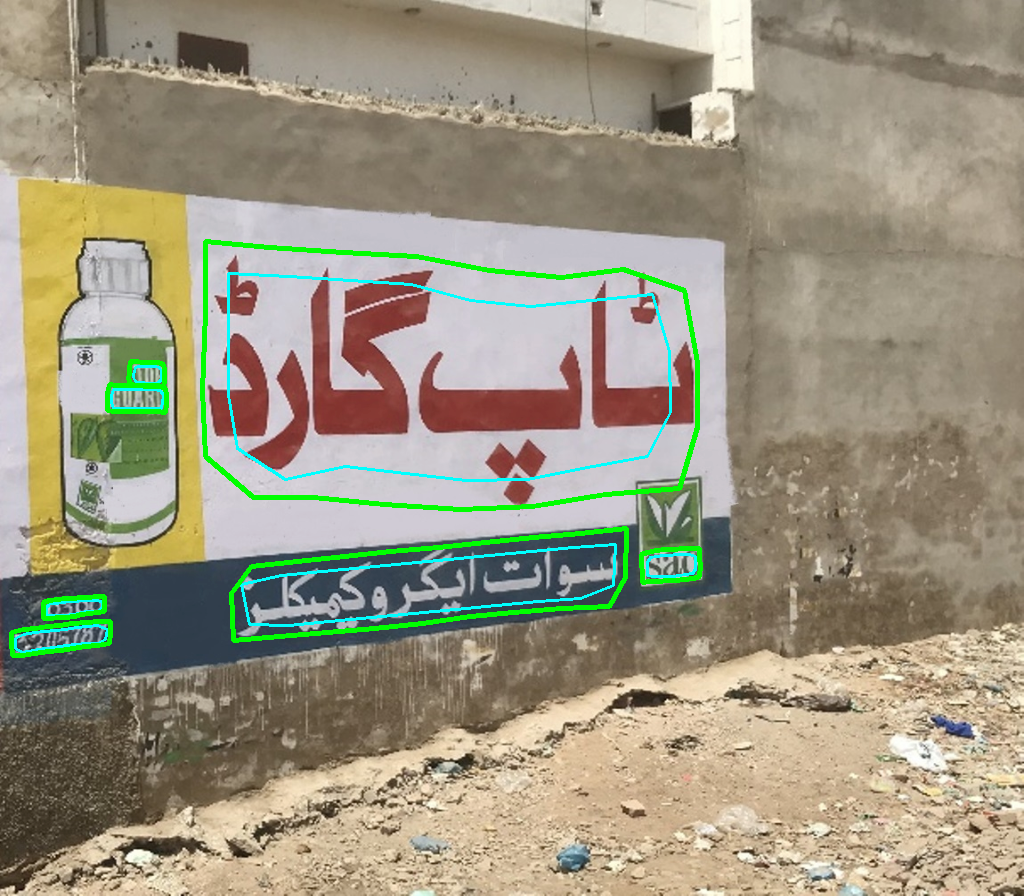
\includegraphics[width=\linewidth]{ITU-Thesis-LaTeX-Template-Updated/figures/holistic 1.png}  
  \end{minipage}
  \begin{minipage}{0.4\textwidth}
    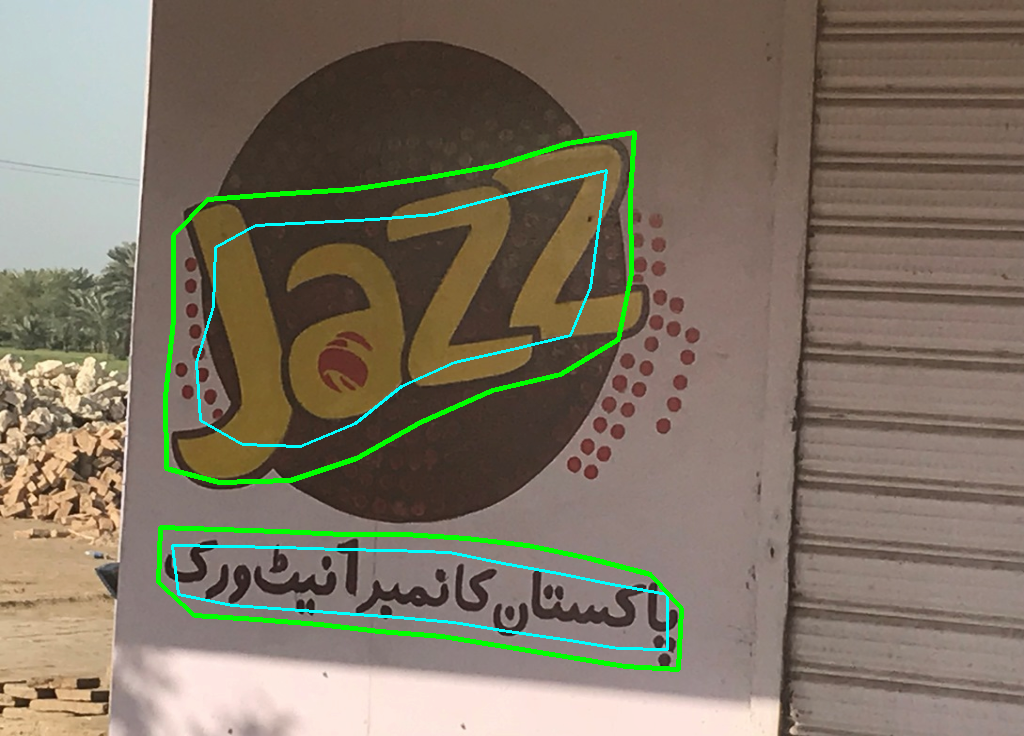
\includegraphics[width=\linewidth]{ITU-Thesis-LaTeX-Template-Updated/figures/hol2.png} 
  \end{minipage}
  \begin{minipage}{0.4\textwidth}
    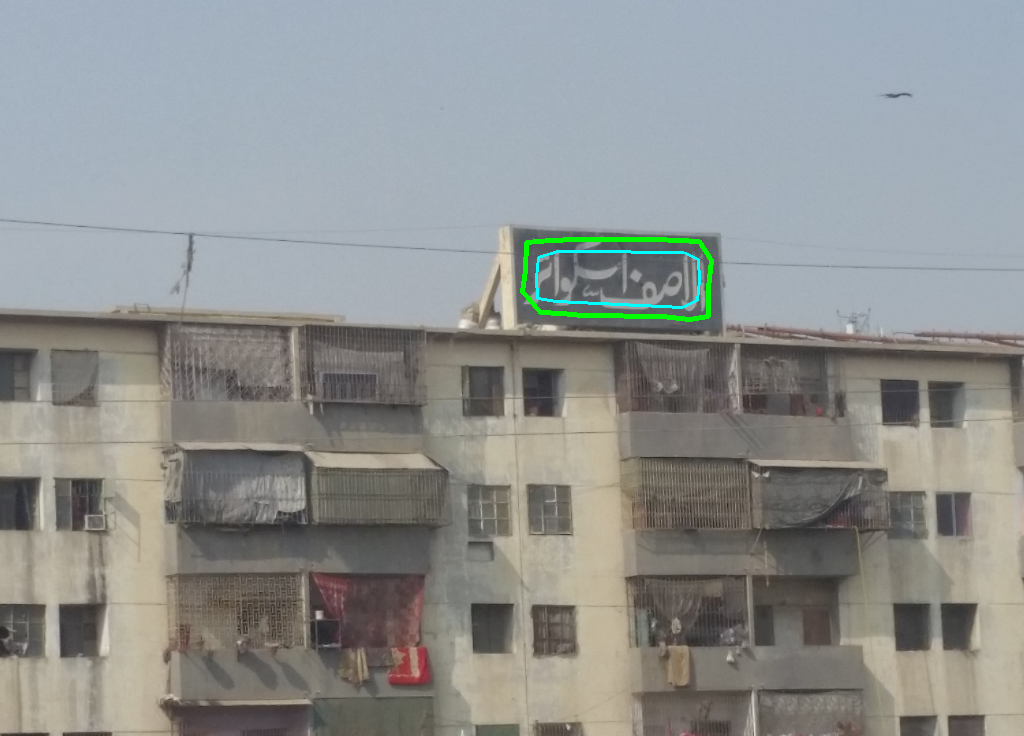
\includegraphics[width=\linewidth]{ITU-Thesis-LaTeX-Template-Updated/figures/hol3.png}
   
  \end{minipage}
  \begin{minipage}{0.4\textwidth}
    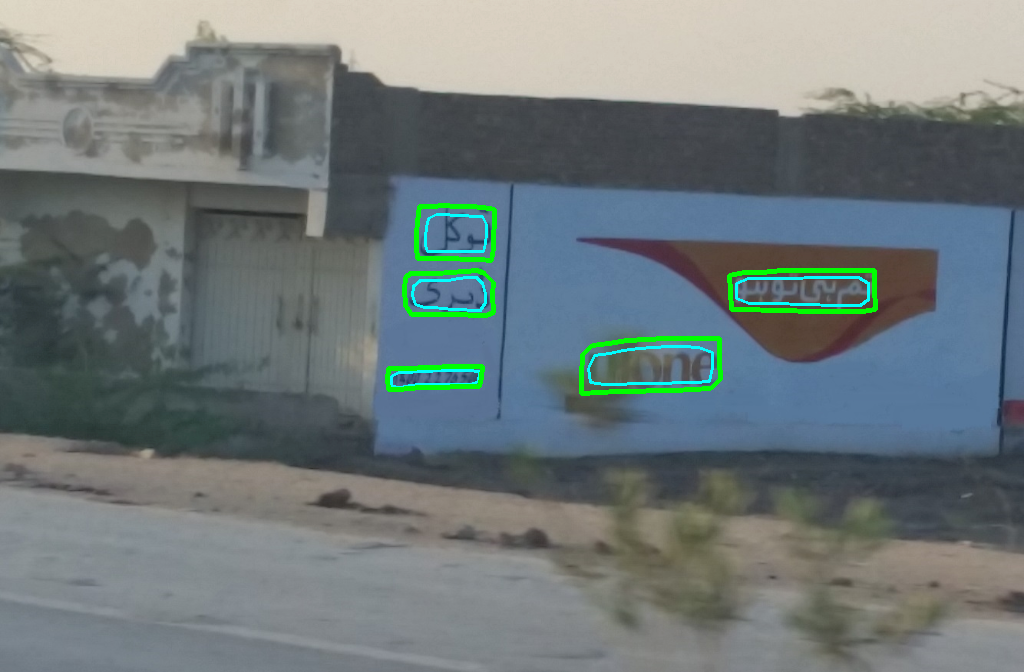
\includegraphics[width=\linewidth]{ITU-Thesis-LaTeX-Template-Updated/figures/hol4.png}
    
  \end{minipage}
  \caption[Hoslistic Performance]{Demonstration of the holistic best performance achieved using GCN (Graph Convolutional Network). These results showcase GCN's superior capabilities in handling diverse and complex data, delivering outstanding overall performance across various tasks and scenarios.}

  \label{fig:holistic}
\end{figure}
\FloatBarrier

In conclusion, our thorough visual model comparison leaves no room for doubt: Graph Convolutional Networks (GCN) stand out as the unequivocal choice for text detection across diverse and challenging scenarios. The combination of GCN's adaptability to multi-oriented text, its precision in detecting arbitrary shapes, and its unmatched robustness amidst complex backgrounds establishes it as the premier option for achieving accurate and reliable text detection results.

Through this research, we have provided compelling evidence that GCN not only outperforms competing models but also offers a holistic solution for text detection in real-world applications. Researchers and practitioners seeking optimal text detection methodologies can confidently turn to GCN as the superior choice.

This structure emphasizes the superior performance of GCN across various critical factors, making a strong case for its selection in text detection applications.

\subsection{Scalability and Efficiency}

An essential consideration in our assessment was the scalability and efficiency of each model. Faster R-CNN and YOLO, established models, offer competitive performance with relatively lower computational demands. They are well-suited for real-time applications and resource-constrained scenarios.

In contrast, the Adaptive Deformation Model, owing to its innovative features such as Graph Convolutional Networks (GCN), presents higher computational requirements. However, it demonstrates the potential for substantial accuracy improvements, particularly valuable in intricate scenarios where both precision and recall are critical.

\subsection{Conclusion}

To conclude, our comparative analysis provides valuable insights into the unique strengths and characteristics of each text detection model. The choice of the most suitable model hinges on the specific requirements of the application. Faster R-CNN, YOLO, and the Adaptive Deformation Model each offer valuable capabilities, and the decision should consider factors like precision-recall trade-offs, robustness to text variability, scalability, and efficiency.

This detailed analysis empowers researchers and practitioners with the insights needed to make informed decisions when selecting a text detection solution for diverse real-world scenarios. By offering a nuanced understanding of each model's performance, this section equips stakeholders to optimize text detection methodologies effectively.




\FloatBarrier

